\documentclass[dvipdfmx,a4paper,11pt]{jsbook}

% 数式
\usepackage{amsmath,amsfonts}
\usepackage[mathcal]{euscript}
\usepackage{mathtools}
\usepackage{xcolor}
\usepackage{xcoffins,calc}
\usepackage{bm}
\usepackage{amsthm}
\usepackage{amssymb}
\usepackage{pgf}
\usepackage{tcolorbox}
\usepackage{titlesec}
\usepackage{ifthen}
\usepackage{mathrsfs}
\usepackage[scr]{rsfso}
\usepackage{relsize}
\usepackage{makeidx}

% 画像
% \usepackage[dvipdfmx]{graphicx,color}

\usepackage[%
dvipdfmx, %欧文ではコメントアウトする
setpagesize=false,
bookmarks=true,
bookmarksdepth=tocdepth,
bookmarksnumbered=true,
colorlinks=true,
linkcolor=blue,
citecolor=blue,
urlcolor=blue,
pdftitle={},
pdfsubject={},
pdfauthor={},
pdfkeywords={}
]{hyperref}

\usepackage{pxjahyper}
\usepackage{tikz}
\usetikzlibrary{intersections,calc,arrows.meta}
\usepackage[truedimen,top=25truemm,bottom=30truemm,hmargin=25truemm]{geometry}
\usepackage{calc}
\usepackage{fancyhdr}
\pagestyle{fancy}


\pagestyle{fancy}
\fancyhf{} % 全てのヘッダーとフッターをクリア
\fancyhead[LE,RO]{\thepage} % 左側の偶数ページと右側の奇数ページにページ番号を表示
\fancyhead[RE]{\leftmark} % 右側の偶数ページに章名を表示
\fancyhead[LO]{\rightmark} % 左側の奇数ページに節名を表示
\renewcommand{\headrulewidth}{0.4pt} % ヘッダーの線の太さを設定
\renewcommand{\footrulewidth}{0pt} % フッターの線の太さを定

% \makeatletter
% \let\old@rule\@rule
% \def\@rule[#1]#2#3{\textcolor{blue}{\old@rule[#1]{#2}{#3}}}
% \makeatother
% \newtcolorbox{mybox}[2][]{enhanced,skin=enhancedlast jigsaw,
% attach boxed title to top left={xshift=-4mm,yshift=-0.5mm},
% fonttitle=\bfseries\sffamily,varwidth boxed title=0.7\linewidth,
% colbacktitle=blue!45!white,colframe=red!50!black,
% interior style={top color=blue!10!white,bottom color=red!10!white},
% boxed title style={empty,arc=0pt,outer arc=0pt,boxrule=0pt},
% underlay boxed title={
% \fill[blue!45!white] (title.north west) -- (title.north east)
% -- +(\tcboxedtitleheight-1mm,-\tcboxedtitleheight+1mm)
% -- ([xshift=4mm,yshift=0.5mm]frame.north east) -- +(0mm,-1mm)
% -- (title.south west) -- cycle;
% \fill[blue!45!white!50!black] ([yshift=-0.5mm]frame.north west)
% -- +(-0.4,0) -- +(0,-0.3) -- cycle;
% \fill[blue!45!white!50!black] ([yshift=-0.5mm]frame.north east)
% -- +(0,-0.3) -- +(0.4,0) -- cycle; },
% title={#2},#1}

% chapter 
\titleformat{\chapter}[block]
{}{}{0pt}{
\ifthenelse{\value{chapter}=0}{}
{\vspace*{-2cm}}\fontsize{27pt}{30pt}\selectfont\filleft
}[
\ifthenelse{\value{chapter}=0}{\hrule}{\titleline{
\hspace{225pt}
\begin{tikzpicture}
\draw [thick,line width = 0.4pt] (0,0) -- (7.5cm,0);
\draw [thick,line width = 0.4pt] (6.5cm,2cm)-- (6.5cm,-1cm);
% \draw [line width = 0.4pt] (6.5cm,1cm) -- (6.5cm,-1cm);
\end{tikzpicture}}}
\Large{\filleft \ifthenelse{\value{chapter}=0}{}{\vspace*{-1cm}第 \thechapter 章}}
]



\makeatletter
\def\Section{\@ifstar{\@Section[2pt]}{\@Section[\z@]}}
%
\def\@Section[#1]#2{\ifdim #1<1pt\refstepcounter{section}\fi%
\section*{\nopagebreak[4] \vskip.5pc%
\ifdim #1<1pt%
\addcontentsline{toc}{section}{\protect\numberline{\thesection}#2}%
\quad \textbf{\thesection~} \fi \raisebox{-1.5ex}[0pt][0pt]{\color[rgb]{0.6,0.8,1}{\rule{3mm}{2em}}} #2\nopagebreak[4]%
\vskip.25pc \hrule\@height 1pt\nopagebreak[4] \vskip1pc}}
\makeatother

% % 定理環境の設定
\tcbuselibrary{skins, breakable, theorems}
\usepackage{cleveref}
% \newcommand{\kara}{}
% \newtcolorbox[auto counter, number within = section, crefname = {Def.}{Defs.}]{definition}[3][]{enhanced, breakable = true, fonttitle = \bfseries,title = Def.~\thetcbcounter~\if #2\kara \else (#2) \fi, #1, label = the:#3, boxrule=0pt, frame hidden, borderline west={4pt}{0pt}{green!75!black},
% colback=green!10!white,sharp corners}



% \newtheorem{theorem}{Theorem}[section]
% \tcolorboxenvironment{theorem}{
%   colback=blue!5!white,
%   boxrule=0pt,
%   boxsep=1pt,
%   left=2pt,right=2pt,top=2pt,bottom=2pt,
%   oversize=2pt,
%   sharp corners,
%   before skip=\topsep,
%   after skip=\topsep,
% }




\renewcommand{\qedsymbol}{$\blacksquare$}
\newcommand{\Claim}[1]{\underline{\textbf{Claim#1.}}}

\newcommand{\kara}{}%
\newcounter{totalcounter}
\renewcommand{\thetotalcounter}{\thechapter.\thesection.\arabic{totalcounter}}
\newcounter{defcounter}
\renewcommand{\thedefcounter}{\thechapter.\thesection.\arabic{defcounter}}

\NewTotalTColorBox[use counter = defcounter, number within = section]{\Definition}{ +m }{ 
notitle,
colback=green!5!white,
frame hidden,
boxrule=0pt,
enhanced,
sharp corners,
borderline west={4pt}{0pt}{green!50!black},
breakable = true,
label = {Def:\thedefcounter},
}{
\textcolor{green!50!black}{
    \sffamily
    \textbf{Definition~\thetcbcounter.}%k
}%
#1
}

\NewTotalTColorBox{\Remark}{ +m +m }{ 
notitle,
colback=yellow!5!white,
colbacklower=white,
frame hidden,
boxrule=0pt,
bicolor,
sharp corners,
borderline west={4pt}{0pt}{yellow!50!black},
%fontupper=\sffamily,
breakable = true,
label = {Rem:\thetotalcounter},
}{
\textcolor{yellow!50!black}{
    \sffamily
    \textbf{Remark~.}%
}%
#1
\if #2\kara \else 
\tcblower%
\textcolor{yellow!50!black}{
    \sffamily
    \textbf{Proof.}%
}%
#2
\qedsymbol
\fi
}

\NewTotalTColorBox[use counter = totalcounter, number within = section]{\Lemma}{ +m +m }{ 
notitle,
colback=orange!5!white,
colbacklower=white,
frame hidden,
boxrule=0pt,
bicolor,
sharp corners,
borderline west={4pt}{0pt}{orange!50!black},
fontupper=\sffamily,
breakable = true,
label = {Lem:\thetotalcounter},
}{
\textcolor{orange!50!black}{
    \sffamily
    \textbf{Lemma~\thetcbcounter.}%
}%
#1
\if #2\kara \else 
\tcblower%
\textcolor{orange!50!black}{
    \sffamily
    \textbf{Proof.}%
}%
#2
\qedsymbol
\fi
}


\NewTotalTColorBox[use counter = totalcounter, number within = section]{\Theorem}{ +m +m }{ 
notitle,
colback=blue!5!white,
colbacklower=white,
frame hidden,
boxrule=0pt,
bicolor,
sharp corners,
borderline west={4pt}{0pt}{blue!50!black},
fontupper=\sffamily,
breakable = true,
label = {Thm:\thetotalcounter},
}{
\textcolor{blue!50!black}{
    \sffamily
    \textbf{Theorem~\thetcbcounter.}%
}%
#1
\if #2\kara \else 
\tcblower%
\textcolor{blue!50!black}{
    \sffamily
    \textbf{Proof.}%
}%
#2
\qedsymbol
\fi
}

\NewTotalTColorBox[use counter = totalcounter, number within = section]{\Example}{ +m +m }{ 
notitle,
colback=cyan!5!white,
colbacklower=white,
frame hidden,
boxrule=0pt,
bicolor,
sharp corners,
borderline west={4pt}{0pt}{cyan!50!black},
%fontupper=\sffamily,
breakable = true,
label = {Ex:\thetotalcounter},
}{
\textcolor{cyan!50!black}{
    \sffamily
    \textbf{Example~\thetcbcounter.}%
}%
#1
\if #2\kara \else
\tcblower%
\textcolor{cyan!50!black}{
    \sffamily
    \textbf{Proof.}%
}%
#2
\qedsymbol
\fi
}

\NewTotalTColorBox[use counter = totalcounter, number within = section]{\Proposition}{ +m +m }{ 
notitle,
colback=red!5!white,
colbacklower=white,
frame hidden,
boxrule=0pt,
bicolor,
sharp corners,
borderline west={4pt}{0pt}{red!50!black},
fontupper=\sffamily,
breakable = true,
label = {Prop:\thetotalcounter},
}{
\textcolor{red!50!black}{
    \sffamily
    \textbf{Proposition~\thetcbcounter.}%
}%
#1
\if #2\kara \else 
\tcblower%
\textcolor{red!50!black}{
    \sffamily
    \textbf{Proof.}%
}%
#2
\qedsymbol
\fi
}
\NewTotalTColorBox[use counter = totalcounter, number within = section]{\Corollary}{ +m +m }{ 
notitle,
colback=darkgray!5!white,
colbacklower=white,
frame hidden,
boxrule=0pt,
bicolor,
sharp corners,
borderline west={4pt}{0pt}{darkgray!50!black},
fontupper=\sffamily,
breakable = true,
label = {Cor:\thetotalcounter},
}{
\textcolor{darkgray!50!black}{
    \sffamily
    \textbf{Corollary~\thetcbcounter.}%
}%
#1
\if #2\kara \else 
\tcblower%
\textcolor{darkgray!50!black}{
    \sffamily
    \textbf{Proof.}%
}%
#2
\qedsymbol
\fi
}
\definecolor{background}{HTML}{FCF9EE}
\definecolor{linecolor}{HTML}{581810}
\newtcolorbox{conditionbox}{enhanced,
  boxsep=0.25ex,
  arc=0mm,
  borderline west={1pt}{-0.5pt}{linecolor},
  borderline east={1pt}{-0.5pt}{linecolor},
  colback=background,
  colframe=background,
  overlay={
    \foreach \n in {north east,north west,south east,south west}
      {%
      \draw [linecolor, fill=linecolor] (frame.\n) circle (2pt);
      };
  }
}

% \newtcbtheorem[use counter from = theorem]{mythm}{Theorem}%
% {
%   colback=white, % ボックス内の背景色
%   colframe=black, % フレームの色
%   fonttitle=\bfseries, % タイトルのフォント
% }{thm}

% % 証明環境の設定
% \newtcbtheorem[use counter from = theorem]{mypf}{Proof}%
% {
%   colback=white, 
%   colframe=black, 
%   fonttitle=\bfseries
% }{prf}

% % 定義環境の設定
% \newtcbtheorem[use counter from = theorem]{mydef}{Definition}%
% {
%   colback=white, 
%   colframe=black, 
%   fonttitle=\bfseries
% }{def}

\newtcolorbox{mybox}{
enhanced,
boxrule=0pt,frame hidden,
borderline west={4pt}{0pt}{green!75!black},
colback=green!10!white,
sharp corners
}

\newcommand{\mysetminusD}{\hbox{\tikz{\draw[line width=0.6pt,line cap=round] (3pt,0) -- (0,6pt);}}}
\newcommand{\mysetminusT}{\mysetminusD}
\newcommand{\mysetminusS}{\hbox{\tikz{\draw[line width=0.45pt,line cap=round] (2pt,0) -- (0,4pt);}}}
\newcommand{\mysetminusSS}{\hbox{\tikz{\draw[line width=0.4pt,line cap=round] (1.5pt,0) -- (0,3pt);}}}

\newcommand{\mysetminus}{\mathbin{\mathchoice{\mysetminusD}{\mysetminusT}{\mysetminusS}{\mysetminusSS}}}

\newcommand{\defi}{\stackrel{\mathrm{def}}{\equiv}}
\renewcommand{\ker}[1]{\mathrm{Ker}\, #1}
\newcommand{\im}[1]{\mathrm{Im}\, #1}
\newcommand{\coker}[1]{\mathrm{Coker}\, #1}
\renewcommand{\hom}[3]{\mathrm{Hom}_{#1}(#2,#3)}
\newcommand{\spec}[1]{\mathrm{Spec}\, #1}

\makeindex

\begin{document}

% \setlength{\topmargin}{-20truemm}
% \setlength{\headheight}{0pt}
% \setlength{\headsep}{0pt}
\setlength{\footskip}{20truemm}



% \setlength{\@tempdima}{1pt*\ratio{\dimexpr\textheight/\@lines}{\baselineskip}}
% \renewcommand{\baselinestretch}{\strip@pt\@tempdima}\selectfont

\makeatletter
\newcount\@chars\newcount\@lines
\@chars=40                      % 1行の文字数
\@lines=40                      % 1ページの行数

\newdimen\@kanjiskip
\@kanjiskip=\dimexpr(\textwidth-1zw*\@chars)/\numexpr\@chars-1
\newdimen\@@kanjiskip
\@@kanjiskip=\dimexpr\@kanjiskip/10

\baselineskip=\dimexpr\textheight/\@lines
\kanjiskip=\@kanjiskip plus \@@kanjiskip minus \@@kanjiskip
\parindent=\dimexpr 1zw+2truept
\parindent=\dimexpr\parindent+\@kanjiskip
\makeatother

% ↑は貼り付けただけなのでわからない.



\title{代数幾何まとめノート}
\date{\today}
\author{Fefr}
\maketitle



\setcounter{tocdepth}{2}
\tableofcontents
\clearpage
%--------------------本文--------------------%

\chapter{Scheme}

\Section{Zariski Topology}
$\spec{A}$を幾何的な対象に昇華するために,位相を導入しよう.まず,環$A$のイデアル$I$に対して
\begin{align*}
  V(I) &= \{\mathfrak{p} \in \spec{A}\mid I\subset \mathfrak{p}\}\\
  D(I) &= \spec{A}\mysetminus V(I) = \{\mathfrak{p} \in \spec{A}\mid I\not\subset \mathfrak{p}\}
\end{align*}
更に,$f\in A$に対して
\begin{align*}
  V(f) &= \{\mathfrak{p} \in \spec{A}\mid Af \subset \mathfrak{p}\}\\
  D(f) &= \spec{A}\mysetminus V(Af) = \{\mathfrak{p} \in \spec{A}\mid Af \not\subset \mathfrak{p}\}
\end{align*}
と定義する.
また,$Af\subset \mathfrak{p}$より$af\in Af$は$af\in \mathfrak{p}$なので,$a=1$とすれば$f\in \mathfrak{p}$がわかり,
イデアルの定義より,
\begin{align*}
  V(f) &= \{\mathfrak{p} \in \spec{A} \mid f \in \mathfrak{p}\}\\
  D(f) &= \{\mathfrak{p} \in \spec{A} \mid f \notin \mathfrak{p}\}
\end{align*}
がわかる.次に$\{D(f)\}_{f\in A}$を開集合族とする位相が定まることを示そう.

\Proposition{
  ああああ
}{}

\Section{Algebraic Sets}
atodekakuyo

\Section{Sheaves}
\Definition{
$X$を位相空間とする.$X$上の(アーベル群の)\textbf{前層}(presheaf)$\, \mathcal{F}$とは
次のデータ
\begin{center}
  \begin{itemize}
    \item[---] $U$を任意の$X$の開集合に対して$\mathcal{F}(U)$はアーベル群.
    \item[---] 制限写像(restriction map)と言われる群準同型
          $\rho_{U,V}:\mathcal{F}(U) \to \mathcal{F}(V)$が任意の開集合$V\subset U$に対して存在する.
  \end{itemize}
\end{center}
そして次の条件を満たす.
\begin{itemize}
  \item[(1)] $\rho_{U,U} = \text{id}_{\mathcal{F}(U)}$
  \item[(2)] 任意の開集合$W\subset V \subset U$に対して$\rho_{U,W}=\rho_{V,W}\circ \rho_{U,V}$となる.
\end{itemize}
}
$s\in \mathcal{F}(U)$を$U$上の$\mathcal{F}$の\textbf{切断}(section)という.
また,$\rho_{U,V}(s)\in \mathcal{F}(V)$を$s|_{V}$と書いて$s$の$V$への制限という.\\
また,単に$\mathcal{F,G,H,}\dots$などと書いたら(前)層を表すことや、$\rho$と書いたら制限写像を意味する。
また,どの(前)層の制限写像かを明示するため,例えば,$\rho_{U,V}^{\mathcal{F}}$などと書くことがある。
\Definition{
前層$\mathcal{F}$が層(sheaf)とは次の条件を満たすことをいう.
\begin{itemize}
  \item[(4)] (Uniqueness) $U$を$X$の開集合とし$\{U_{i}\}_{i}$をその開被覆とする.
        $s\in \mathcal{F}(U)$が任意の$i$に対して$s|_{U_{i}}=0$ならば$s=0$
  \item[(5)] (Glueing local sections) 上の状況で,$s_i \in \mathcal{F}(U_i)$が
        $s_{i}|_{U_{i} \cap U_{j}} = s_{j}|_{U_{i} \cap U_{j}}$を満たすならば,$s|_{U_{i}} = s_{i}$を満たす$s\in \mathcal{F}(U)$が存在する.
\end{itemize}
}
\Remark{
$\mathcal{F}$が層ならば$\mathcal{F}(\varnothing) = 0$となる.
}{}
\Example{
$X$を位相空間とする.\\
$\mathcal{C}_{X}^{0}$を$X$の開集合$U$に対して$U\to \mathbf{C}$なる連続写像全体の集合$\mathcal{C}_{X}^{0}(U)$を対応させるものとし,制限写像を普通の制限とする.
\begin{equation*}
  \mathcal{C}_{X}^{0}(U) = \left\{ f:U \to \mathbf{C} \mid f\text{ is continuous} \right\}
\end{equation*}
すると,$\mathcal{C}_{X}^{0}$は$X$上の層となる.
}{
$V \subset U$なる開集合$U,V$に対して$U$上の連続写像$f\in \mathcal{C}_{X}^{0}(U)$を$V$に制限することによって得られる
$V$上の連続写像を$\rho_{U,V}(f)(=f|_{V})$と書く.すると,これは$\mathbf{C}$上のベクトル空間($\mathbf{C}$上の関数空間)
の準同型$\rho_{U,V}:\mathcal{C}_{X}^{0}(U) \to \mathcal{C}_{X}^{0}(V)$となる.つまり$(\mathcal{C}_{X}^{0},\rho)$は前層となる.\\
また,(4)を満たすのは明らかで.(5)もすぐに成り立つことがわかる.$\{U_{i}\}_{i}$を$U$の開被覆とする.$f_{i} \in \mathcal{C}_{X}^{0}(U_{i})$が
$f_{i}|_{U_{i} \cap U_{j}} = f_{j}|_{U_{i} \cap U_{j}}$を満たすとする.するとそれらを張り合わせた関数を$f$とすればこれは
$f\in \mathcal{C}_{X}^{0}(U)$であり,$f|_{U_{i}}=f_{i}$となる.よって$(\mathcal{C}_{X}^{0},\rho)$は層となる.これを連続写像が成す層という.
}
\Example{
$X$を位相空間とする.\\
$A$を自明でないアーベル群とする.$\mathcal{A}_{X}$を$X$の空でない開集合$U$に対して$\mathcal{A}_{X}(U)=A$に,
空集合$\varnothing$に対して$\mathcal{A}_{X}(\varnothing) = 0$に対応させるものとし,
制限写像を空でない開集合$V \subset U$に対して$\rho_{U,V}=\text{id}_{A}$とし,$\rho_{U,\varnothing} = 0$とする.\\
すると,$(\mathcal{A}_{X},\rho)$は$X$上の前層にはなるが,一般に層とはならない.\\
}{
例えば,$X$が連結でないとすると,非交差な開集合$U,V$があって$X=U\cup V$とかける.すると$\{U,V\}$は$X$の開被覆となる.
$s_{U} \in \mathcal{A}_{X}(U)=A$が$s_{U}|_{U\cap V} = s_{U}|_{\varnothing} = 0 = s_{V}|_{U \cap V}$
を満たすとする.このとき,任意の$s \in \mathcal{A}_{X}(X)=A$で$s|_{U}=s|_{V}=s$となり層とならない.
}

\Example{
(skyscraper sheaf)\\
$X$を位相空間、$A$をアーベル群とする。$p\in X$に対して$i_{p} : \{p\} \hookrightarrow X$を包含写像とする。
このとき$i_{p,*}\mathcal{A}$を
\begin{equation*}
  i_{p,*}\mathcal{A}(U) = \left\{
  \begin{alignedat}{2}
      & A \qquad & p \in U    \\
      & 1 \qquad & p \notin U
  \end{alignedat}
  \right.
\end{equation*}
と定義する。これは層になる。
}{}




\Definition{
  位相空間$X$上の前層$\mathcal{F}$と$x\in X$に対して,$x$での$\mathcal{F}$の\textbf{茎(stalk)}$\mathcal{F}_{x}$という群が定義できる.
  \begin{equation*}
    \mathcal{F}_{x} = \varinjlim_{U \ni x}\mathcal{F}(U)
  \end{equation*}
  ただし,$U$は$x$の開近傍をすべてを回る.$U$上の切断$s\in \mathcal{F}(U)$に対して
  $x\in U$の茎$\mathcal{F}_{x}$への自然な群準同型の像を$s_{x}$と書いて,$x$での$s$の\textbf{芽(germ)}という.
}
\Remark{
  ここで,$\mathcal{F}_{x}$は$x$近傍の情報を持っていると言える.実際,
  \begin{equation*}
    \mathcal{F}_{x} = \left. \bigsqcup_{i}U_{i}\right/{\mathlarger{\sim}}\qquad \cdots (*)
  \end{equation*}
  ここで,同値関係は
  \begin{equation*}
    (t,U)\sim (s,V) \defi \exists W\subset U,V,x\in W\ \text{s.t.}\ t|_{W}=s|_{W} 
  \end{equation*}
  である.ただし,$(t,U)$とは$x$の開近傍$U$で$t\in \mathcal{F}(U)$という意味である.また$(*)$
  を見れば分かるように,$\mathcal{F}_{x}$の任意の元はある$x$近傍$U$上の切断$s\in \mathcal{F}(U)$
  の芽である.
}{}

\Proposition{
  層の定義の(4),(5)を次の列が完全系列であるとすることができる.
  \begin{equation*}
    C^{\bullet}(\mathcal{U},\mathcal{F}) : 0 \longrightarrow \mathcal{F}(U) \stackrel{d_{0}}{\longrightarrow} \prod_{i}\mathcal{F}(U_{i}) \stackrel{d_{1}}{\longrightarrow} \prod_{i}\mathcal{F}(U_{i}\cap U_{j})
  \end{equation*}
  ただし,$\mathcal{U}$は開集合$U$の開被覆で$\mathcal{U} = \{U_{i}\}_{i}$.\\
  $d_{0} : s\mapsto (s|_{U_{i}})_{i},d_{1}: (s_{i})_{i} \mapsto (s_{i}|_{U_{i}\cap U_{j}} - s_{j}|_{U_{i}\cap U_{j}})_{i,j}$
}{
}

\Lemma{
$\mathcal{F}$を$X$上の層とする.$s,t \in \mathcal{F}(X)$が任意の$x \in X$に対して$s_{x} = t_{x}$ならば$s=t$
}{
差を考えれば$t=0$のときを考えればいい.$s_{x}=0\ (\forall x\in X)$とすると,$x$の開近傍$U_{x}$があって$s|_{U_{x}}=0$となる.$\{U_{x}\}_{x\in U_{x}}$は$X$の開被覆なので,$s=0$となる.
}
\Definition{
$X$上の2つの前層$\mathcal{F,G}$とする.\textbf{前層の射}$\alpha:\mathcal{F} \to \mathcal{G}$
とは,$X$の開集合$U$に対して群準同型$\alpha(U):\mathcal{F}(U) \to \mathcal{G}(U)$があって,
任意の開集合の組$V\subset U$に対して$\alpha(V)\circ \rho_{U,V}^{\mathcal{F}} = \rho_{U,V}^{\mathcal{G}}\circ \alpha(U)$を満たすことをいう.\\
$X$の任意の開集合$U$に対して$\alpha(U)$が単射ならば$\alpha$は単射であるという.(全射はうまくいかんっぽい?)
}

$\alpha:\mathcal{F} \to \mathcal{G}$を$X$上の前層の射とする.任意の$x \in X$に対して
$\alpha$から自然に誘導される群準同型$\alpha_{x}:\mathcal{F}_{x} \to \mathcal{G}_{x}$で
$(\alpha(U)(s))_{x} = \alpha_{x}(s_{x})$が$X$の任意の開集合$U,s\in \mathcal{F}(U),x\in U$で
成り立つものが取れる.\\
$\alpha_{x}$が任意の$x\in X$で全射なら$\alpha$が全射であるという.

\Example{
  $X=\mathbf{C} \mysetminus \{0\}$とし$\mathcal{F}$を$X$上の正則関数がなす層とし,
  $\mathcal{G}$を$X$上の双正則関数のなす層とする.今,任意の開集合$U$と任意の$f\in \mathcal{F}(U)$に対して$\alpha(U)(f) = \exp(f)$で定義される層の射$\alpha:\mathcal{F} \to \mathcal{G}$
  が全射であることはよく知られている.しかし$\alpha(X):\mathcal{F}(X) \to \mathcal{G}(X)$は
  全射ではない.例えば恒等写像は$\exp(f)$と書けない.
}{}
\Proposition{
  $\alpha:\mathcal{F} \to \mathcal{G}$を$X$上の層の射とする.
  \begin{center}
    $\alpha$が同型$\Leftrightarrow$ $\alpha_{x}$が同型$(\forall x \in X)$
  \end{center}
}{}
\Theorem{
位相空間$X$上の前層$\mathcal{F}$に対して,前層$\mathcal{F}$の層化(sheafification)$\mathcal{F}^{\dagger}$は存在する.
}{
$X$の開集合$U$に対して
\begin{equation*}
  \mathcal{F}^{\dagger}(U) = \left\{\sigma: U \to \prod_{x\in U} \mathcal{F}_{x}\, \middle|\,
  \begin{aligned}
    \forall x\in U,x\in \exists V\subset U:\text{open},\exists s \in \mathcal{F}(V)\, \text{s.t.}\, \sigma(y) = s_{y}\, (\forall y \in V)
  \end{aligned}
  \right\}
\end{equation*}
とする.ただし,$\sigma$は任意の$x\in U$に対して$\sigma(x) \in \mathcal{F}_{x}$とする.
また,$V \subset U$なる開集合に対し,
$$
  \begin{array}{rccc}
    \rho_{U,V}^{\mathcal{F}^{\dagger}}: & \mathcal{F}^{\dagger}(U) & \longrightarrow & \mathcal{F}^{\dagger}(V) \\
                                        & \rotatebox{90}{$\in$}    &                 & \rotatebox{90}{$\in$}    \\
                                        & \sigma                   & \longmapsto     & \sigma|_{V}
  \end{array}
$$
が定義できる.実際,任意の$x\in V$をとる.$V \subset U$であり,
$\sigma \in \mathcal{F}^{\dagger}(U)$より
\begin{center}
  $x\in \exists U_{0} \subset U$:open,$\exists s \in \mathcal{F}(U_{0})$\, s.t.\, $\sigma(y)=s_{y}\, (\forall y\in U_{0})$
\end{center}
$V_{0} = U_{0} \cap V,\quad t = s|_{V_{0}}$とすると任意の$y\in V_{0}$に対して
\begin{equation*}
  \sigma(y)=\sigma|_{V}(y)=s_{y}
\end{equation*}
さらに帰納極限の定義から
\begin{equation*}
  \sigma|_{V}(y)=t_{y}
\end{equation*}
次に$\mathcal{F}^{\dagger}(U)$がアーベル群,つまり
$\sigma,\tau \in \mathcal{F}^{\dagger}(U)$ならば$\sigma+\tau \in \mathcal{F}^{\dagger}(U)$
を示そう.\\
$\sigma,\tau \in \mathcal{F}^{\dagger}(U)$より任意の$x\in U$に対して
\begin{align*}
    & x\in \exists U_{0} \subset U:\mathrm{open},\exists s \in \mathcal{F}(U_{0})\ \mathrm{s.t.}\
  \sigma(y) = s_{y}\ (\forall y \in U_{0})                                                       \\
    & x\in \exists V_{0} \subset U:\mathrm{open},\exists t \in \mathcal{F}(V_{0})\ \mathrm{s.t.}\
  \tau(z) = t_{z}\ (\forall z \in V_{0})
\end{align*}
を満たす.いま$W = U_{0} \cap V_{0},s' = s|_{W},t' = t|_{W}$とすると,
\begin{align*}
  x\in W \subset U:\mathrm{open}, s',t' \in \mathcal{F}(W)\ \mathrm{s.t.}\
  (\sigma + \tau)(y)
    & = \sigma(y) + \tau(y)             \\
    & = s_{y} + t_{y}                   \\
    & = (s + t)_{y} \ (\forall y \in W)
\end{align*}
よって$\sigma + \tau \in \mathcal{F}^{\dagger}(U)$また明らかに可換.
よって$\mathcal{F}^{\dagger}(U)$はアーベル群.\\
また,通常の制限で制限写像を定義しているため,$\mathcal{F}^{\dagger}$は前層となる.\\
更に層となることを示そう.\\
$U$を$X$の開集合とし,$\{U_{i}\}_{i}$をその開被覆とする.$\sigma\in \mathcal{F}^{\dagger}(U)$が
任意の$i$に対して$\sigma|_{U_{i}} = 0$とする.つまり任意の$x \in U_{i}$に対して$\sigma(x) = 0$
とする.$U_{i}$は$U$を被覆するので結局$\sigma = 0$となる.\\
次に,$\sigma_{i} \in \mathcal{F}^{\dagger}(U_{i})$とし,
$\sigma_{i}|_{U_{i} \cap U_{j}} = \sigma_{j}|_{U_{i} \cap U_{j}}$と仮定すると,
$$
  \begin{array}{rccc}
    \sigma : & U                     & \longrightarrow & \displaystyle \prod_{x\in U}\mathcal{F}_{x} \\
              & \rotatebox{90}{$\in$} &                 & \rotatebox{90}{$\in$}                       \\
              & x                     & \longmapsto     & \sigma_{i}(x)
  \end{array}
$$
ただし,$x\in U_{i}$.すると,$\sigma$は$\sigma_{i}\in \mathcal{F}^{\dagger}(U_{i})$を張り合わせて作っているので
これは$\sigma \in \mathcal{F}(U)$となることが容易にわかる。よって、$\mathcal{F}^{\dagger}$は層になる。
}



\Proposition{
  層化の射$\theta:\mathcal{F} \to \mathcal{F}^{\dagger}$に対して、
  その茎の射$\theta_{x}:\mathcal{F}_{x} \to \mathcal{F}^{\dagger}_{x}$は同型である。
}{}



\Lemma{
  $\mathcal{F}$を$X$上の層とし、$\mathcal{F}'$を$\mathcal{F}$の部分層とする。
  このとき開集合$U$を$\mathcal{F}(U)/\mathcal{F}'(U)$に対応させるものは前層になる。
}{
  この対応を$\mathcal{G}$とおく。$V \subset U$なる開集合$U,V$をとる。制限写像を
  $$
    \begin{array}{rccc}
      \rho_{U,V}^{\mathcal{G}} : & \mathcal{F}(U)/\mathcal{F}'(U) & \longrightarrow & \mathcal{F}(V)/\mathcal{F}'(V)                \\
                                  & \rotatebox{90}{$\in$}          &                 & \rotatebox{90}{$\in$}                         \\
                                  & s + \mathcal{F}'(U)            & \longmapsto     & \rho_{U,V}^{\mathcal{F}}(s) + \mathcal{F}'(V)
    \end{array}
  $$
  とすると、これはwell-definedである。また、$U\subset V \subset W$なる開集合の組に対して
  \begin{equation*}
    \rho_{U,W}^{\mathcal{G}} = \rho_{V,W}^{\mathcal{G}} \circ \rho_{U,V}^{\mathcal{G}}
  \end{equation*}
  が成り立つことは制限写像の定義から明らかである。よって$\mathcal{G}$は前層。
}
\Definition{
  Lem:\ref{Lem:1.3.8}で定義した前層の層化を$\mathcal{F}/\mathcal{F}'$と書いて、\textbf{商層(quotient shaef)}という。
}
\Definition{
  $\alpha:\mathcal{F} \to \mathcal{G}$を前層の射とする。このとき開集合$U$に対して
  $U \mapsto \ker (\alpha(U))$とするものは$\mathcal{F}$の部分層になる。これを$\ker{\alpha}$と
  書いて、\textbf{$\alpha$の核(kernel of $\alpha$)}という。\\
  更に、$U\mapsto \im (\alpha(U))$は一般には前層となるので、これの層化を$\im \alpha$と書いて、
  \textbf{$\alpha$の像(image of $\alpha$)}という。\\
  また,$U\mapsto \coker (\alpha(U)) = \mathcal{G}(U)/\im (\alpha(U))$は一般には前層となるので,これの層化を$\coker \alpha$と書いて,\textbf{$\alpha$の余核(cokernel of $\alpha$)}という.
}
\Lemma{
$\mathcal{F,G}$を$X$上の層,$\mathcal{F}'$を$\mathcal{F}$の部分層,$\alpha:\mathcal{F} \to \mathcal{G}$を前層の射とする。
このとき、
\begin{align*}
    & (\ker \alpha)_{x} = \ker \alpha_{x}                               \\
    & (\im \alpha)_{x} = \im \alpha_{x}                                 \\
    & (\coker \alpha)_{x} = \coker \alpha_{x}                           \\
    & (\mathcal{F}/\mathcal{F}')_{x} = \mathcal{F}_{x}/\mathcal{F}'_{x}
\end{align*}
が成り立つ。
}{
$\mathcal{Q}(U) = \mathcal{F}(U)/\mathcal{F}'(U)$とおく。\\
このとき、アーベル群の完全列
\begin{center}
  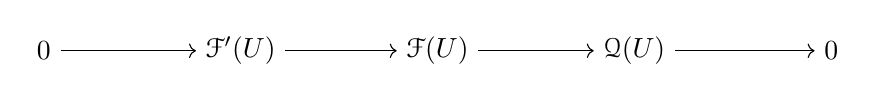
\begin{tikzpicture}[auto]
    \node (03) at (0,-1) {$0$};
    \node (im1) at (2.5,-1) {$\mathcal{F}'(U)$};
    \node (gu) at (5,-1) {$\mathcal{F}(U)$};
    \node (qu) at (7.5,-1) {$\mathcal{Q}(U)$};
    \node (04) at (10,-1) {$0$};

    \draw[->] (03) to (im1);
    \draw[->] (im1) to (gu);
    \draw[->] (gu) to (qu);
    \draw[->] (qu) to (04);
  \end{tikzpicture}
\end{center}
が作れる。帰納極限は完全列を完全列に移すので、またProp:\ref{Prop:1.3.7}より
\begin{center}
  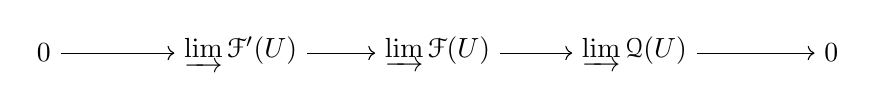
\begin{tikzpicture}[auto]
    \node (03) at (0,-1) {$0$};
    \node (im1) at (2.5,-1) {$\varinjlim \mathcal{F}'(U)$};
    \node (gu) at (5,-1) {$\varinjlim \mathcal{F}(U)$};
    \node (qu) at (7.5,-1) {$\varinjlim \mathcal{Q}(U)$};
    \node (04) at (10,-1) {$0$};

    \draw[->] (03) to (im1);
    \draw[->] (im1) to (gu);
    \draw[->] (gu) to (qu);
    \draw[->] (qu) to (04);
  \end{tikzpicture}
\end{center}
を得る。よって
\begin{center}
  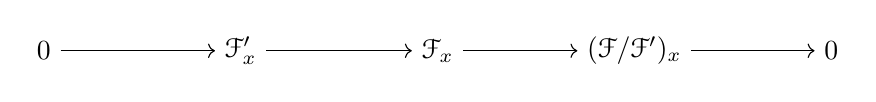
\begin{tikzpicture}[auto]
    \node (03) at (0,-1) {$0$};
    \node (im1) at (2.5,-1) {$\mathcal{F}'_{x}$};
    \node (gu) at (5,-1) {$\mathcal{F}_{x}$};
    \node (qu) at (7.5,-1) {$(\mathcal{F}/\mathcal{F}')_{x}$};
    \node (04) at (10,-1) {$0$};

    \draw[->] (03) to (im1);
    \draw[->] (im1) to (gu);
    \draw[->] (gu) to (qu);
    \draw[->] (qu) to (04);
  \end{tikzpicture}
\end{center}
したがって、
\begin{equation*}
  \mathcal{F}_{x}/\mathcal{F}'_{x} \simeq (\mathcal{F}/\mathcal{F}')_{x}
\end{equation*}
を得る。\\
次に
\begin{align*}
  (\ker \alpha)_{x}
    & = \{s_{x} \in \mathcal{F}_{x} \ |\ \alpha(U)(s) = 0,x\in U:\text{open},s\in \mathcal{F}(U) \}   \\
    & = \{s_{x} \in \mathcal{F}_{x} \ |\ \alpha_{x}(s_{x})=0,x\in U:\text{open},s\in \mathcal{F}(U)\} \\
    & = \ker \alpha_{x}
\end{align*}
を得る。同様に
\begin{align*}
  (\im \alpha)_{x}
    & = \{t_{x} \in \mathcal{G}_{x} \ |\ x\in \exists U:\text{open}, \exists s\in \mathcal{F}(U)\ \text{s.t}\ t = \alpha(U)(s)\} \\
    & = \{(\alpha(U)(s))_{x} \in \mathcal{G}_{x} \ |\ x \in U:\text{open},s\in \mathcal{F}(U)\}                                  \\
    & = \{\alpha_{x}(s_{x}) \in \mathcal{G}_{x}\ |\ s_{x} \in \mathcal{F}_{x}\}                                                  \\
    & = \im \alpha_{x}
\end{align*}
を得る.また,$(\mathcal{F}/\mathcal{F}')_{x} = \mathcal{F}_{x}/\mathcal{F}'_{x}$より
\begin{equation*}
  (\coker \alpha)_{x} = (\mathcal{G}/\im \alpha)_{x} = \mathcal{G}_{x}/\im \alpha_{x} = \coker \alpha_{x}
\end{equation*}
}

\Definition{
  層の列
  \begin{equation*}
    \mathcal{F} \stackrel{\alpha}{\longrightarrow} \mathcal{G} \stackrel{\beta}{\longrightarrow} \mathcal{H}
  \end{equation*}
  が完全とは、$\im \alpha = \ker \beta$が成り立つことをいう。
}
\Proposition{
  層の列に対して次が成り立つ。
  \begin{equation*}
    \mathcal{F} \longrightarrow \mathcal{G} \longrightarrow \mathcal{H}が完全
    \Longleftrightarrow
    任意のx \in Xに対して\mathcal{F}_{x} \longrightarrow \mathcal{G}_{x} \longrightarrow \mathcal{H}_{x}が完全
  \end{equation*}
}{
  明らか。
}

\Definition{
  $X,Y$を位相空間,$f:X\to Y$を連続写像とする。このとき、
  $X$上の層$\mathcal{F}$,$Y$上の層$\mathcal{G}$に対して、新たな$Y$上の層$f_{*}\mathcal{F}$が
  \begin{equation*}
    V \mapsto \mathcal{F}(f^{-1}(V))
  \end{equation*}
  によって定義できる。これを\textbf{$\mathcal{F}$の順像(direct image of $\mathcal{F}$)}という。\\
  また、
  \begin{equation*}
    U \mapsto \varinjlim_{V\supset f(U)}\mathcal{G}(V)
  \end{equation*}
  で定義できる新たな$X$上の前層$f^{\cdot}\mathcal{G}$の層化$f^{*}\mathcal{G}$を\textbf{$\mathcal{G}$の逆像(inverse image of $\mathcal{G}$)}
  という。
}

\Proposition{
  上の状況で
  \begin{equation*}
    (f^{*}\mathcal{G})_{x} = \mathcal{G}_{f(x)} \qquad \forall x \in X
  \end{equation*}
}{
  \begin{equation*}
    (f^{*}\mathcal{G})_{x} = \varinjlim_{x \in U}(f^{*}\mathcal{G})(U) = \varinjlim_{x \in U}\varinjlim_{f(U) \subset V}\mathcal{G}(V) = \mathcal{G}_{f(x)}
  \end{equation*}
  最後の等号は明らか.
}

\Remark{
  $V$を$Y$の開集合とする。このとき自然な単射$i:V \to Y$に対して
  \begin{equation*}
    i^{*}\mathcal{G} = \mathcal{G}|_{V}
  \end{equation*}
  が成り立つ。
}{}
\Proposition{
$f:X \to Y$を位相空間の間の連続写像とし,$\mathcal{F}$を$X$上の層.$\mathcal{G}$を$Y$上の層とする.このとき
\begin{equation*}
  \hom{\text{Sh}(X)}{f^{*}\mathcal{G}}{\mathcal{F}}\simeq \hom{\text{Sh}(Y)}{\mathcal{G}}{f_{*}\mathcal{F}}
\end{equation*}
ただし,$\hom{\mathcal{C}}{X}{Y}$は圏$\mathcal{C}$で$X \to Y$なる射全体を表し,$\text{Sh}(X)$は$X$上の層全体を表す.
}{
層化の普遍性より$\theta:f^{\cdot}\mathcal{G} \to f^{*}\mathcal{G} = (f^{\cdot}\mathcal{G})^{\dagger}$
を層化の射とすると,
$$
  \begin{array}{rccc}
      & \hom{\text{PreSh}(X)}{f^{\cdot}\mathcal{G}}{\mathcal{F}} & \stackrel{\simeq}{\longrightarrow} & \displaystyle \hom{\text{Ph(X)}}{f^{*}\mathcal{G}}{\mathcal{F}} \\
      & \rotatebox{90}{$\in$}                                    &                                    & \rotatebox{90}{$\in$}                                           \\
      & \alpha                                                   & \longmapsto                        & \tilde{\alpha}\circ \theta
  \end{array}
$$
が成り立つ.つまり
\begin{equation*}
  \hom{\text{PreSh}(X)}{f^{\cdot}\mathcal{G}}{\mathcal{F}}\simeq \hom{\text{Sh(Y)}}{\mathcal{G}}{f_{*}\mathcal{F}}
\end{equation*}
を示せばいい.次に$X$上の開集合$U$に対して
\begin{equation*}
  f^{\cdot}\mathcal{G}(U) = \varinjlim_{V\supset f(U)}\mathcal{G}(V)
\end{equation*}
なので,$\varphi \in \hom{\text{PreSh}(X)}{f^{\cdot}\mathcal{G}}{\mathcal{F}}$に対して
\begin{equation*}
  \varphi(U) : \varinjlim_{V\supset f(U)}\mathcal{G}(V) \to \mathcal{F}(U)
\end{equation*}
を与えることは帰納極限の定義より$f(U)\subset V$なる開集合$V$に対して
\begin{equation*}
  \psi'(V) : \mathcal{G}(V) \to \mathcal{F}(U)
\end{equation*}
を$f(U)\subset V' \subset V$ならば,
\begin{equation*}
  \psi'(V) = \psi'(V')\circ \rho^{\mathcal{G}}_{V,V'}
\end{equation*}
となるように与えることである.すなわち$\psi'(V)$は
\begin{equation*}
  \psi(V):\mathcal{G}(V) \to \mathcal{F}(f^{-1}(V))
\end{equation*}
と$\rho^{\mathcal{F}}_{f^{-1}(V),U}$を合成したものである.(帰納系の選び方によらない.)\\
したがって,$\varphi\in \hom{\text{PreSh}(X)}{f^{\cdot}\mathcal{G}}{\mathcal{F}}$を与えることは,$\psi \in \hom{\text{Ph}(Y)}{\mathcal{G}}{f_{*}\mathcal{F}}$を与えることと等しい.
}

\subsection{$\mathfrak{B}$-sheaf}
$\mathfrak{B}$-sheafはアフィンスキームの構成にも必要な概念で,ラフに言えばすべての開集合$U$に対して$\mathcal{F}(U)$が定まっているものではなく,
開基$\mathfrak{B}$の元$U$に対してだけ定まっている層を$\mathfrak{B}$-sheafという.

\Definition{
  位相空間$X$の\textbf{開基$\mathfrak{B}$が有限交叉で閉じている}とは,任意の$U,V\in \mathfrak{B}$に対して$U\cap V \in \mathfrak{B}$が成り立つことをいう. 
}

\Example{
  環$A$の素イデアルの集合$\spec{A}$の基本開集合による開基$\{D(f)\}_{f\in A}$は有限交叉で閉じている.
}{}

\Definition{
  $X$を位相空間.$\mathfrak{B}$をその開基とする.このとき$\mathcal{F}$が
  \textbf{$\mathfrak{B}$-前層($\mathfrak{B}$-presheaf)}であるとは,
  \begin{itemize}
    \item[---] $U\in \mathcal{B}$に対して$\mathcal{F}(U)$はアーベル群.
    \item[---] $V\subset U \in \mathcal{B}$に対して群準同型$\rho_{U,V}:\mathcal{F}(U) \to \mathcal{F}(V)$が定まる.
  \end{itemize}
  で,
  \begin{itemize}
    \item[(1)] $\rho_{U,U} = \text{id}_{\mathcal{F}(U)}$
    \item[(2)] 任意の開集合$W\subset V \subset U$に対して$\rho_{U,W} = \rho_{V,W}\circ \rho_{U,V}$となる.
  \end{itemize}
  を満たすときをいう.
}

\Definition{
  $\mathfrak{B}$が有限交叉で閉じているとする.このとき$\mathfrak{B}$-前層が層の条件を満たすとき
  \textbf{$\mathfrak{B}$-層($\mathfrak{B}$-sheaf)}という.
}

\Proposition{
  $\mathcal{F}$を$\mathfrak{B}$-前層とする.このとき,任意の開集合$V$に対して
  \begin{align*}
    \mathcal{F}(V)
      & = \varprojlim_{\substack{U\in \mathcal{B}                  \\ U\subset V}}\mathcal{F}(U)\\
      & = \left\{(s_{U})_{U} \in \prod_{\substack{U\in \mathcal{B} \\ U \subset V}} \mathcal{F}(U) \ \biggl|\
    \forall U' \subset U \in \mathcal{B}, s_{U}|_{U'}=s_{U'} \right\}
  \end{align*}
  制限写像は射影極限から誘導される射である.
  \begin{center}
    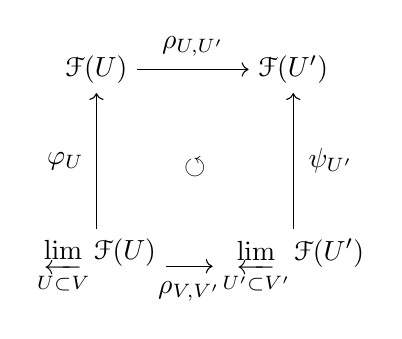
\begin{tikzpicture}[auto]
      \node (X1) at (0,0) {$\mathcal{F}(U)$};
      \node (X2) at (0,-2.5) {$\displaystyle \varprojlim_{U\subset V}\mathcal{F}(U)$};
      \node (Y1) at (2.5,0) {$\mathcal{F}(U')$};
      \node (Y2) at (2.5,-2.5) {$\displaystyle \varprojlim_{U'\subset V'}\mathcal{F}(U')$};
      \node (ci) at (1.25,-1.25) {$\circlearrowleft$};
  
      \draw[->] (X1) to node[yshift = -6pt,label=above:$\rho_{U,U'}$] () {} (Y1);
      \draw[->] (X2) to node[xshift = 6pt, label=left:$\varphi_{U}$] () {} (X1);
      \draw[->] (X2) to node[yshift = -2pt,label=below:$\rho_{V,V'}$] () {} (Y2);
      \draw[->] (Y2) to node[xshift = 2pt,label=right:$\psi_{U'}$] () {} (Y1);
    \end{tikzpicture}
  \end{center}
  するとこれは前層になる.
}{}

\Proposition{
  更に,$\mathfrak{B}$が有限交叉で閉じているなら,層になる.
}{
  任意の開集合$V$に対してその開被覆$\{V_{i}\}_{i}$を取る.ただし$V_{i} \in \mathfrak{B}$とする.\\
  \Claim{ (4)(Uniqueness)が成立する}\\
  $s\in \mathcal{F}(V)$が任意の$i$に対して$s|_{V_{i}} = 0$とする.今定義から$s=0$とは
  $U\subset V$なる任意の$U\in \mathfrak{B}$に対して$s_{U}\in \mathcal{F}(U)$が$0$であること
  である.実際$V$の開被覆から$U$の開被覆$\{U\cap V_{i}\}_{i} \subset \mathfrak{B}$を得る.
  また任意の$i$に対して$U\cap V_{i} \subset V_{i}$より$s|_{V_{i}}|_{U\cap V_{i}} = s|_{U\cap V_{i}} = 0$となる.従って任意の$i$に対して$s_{U}|_{U\cap V_{i}} = 0$となる.
  今$\mathcal{F}$は$\mathfrak{B}$-sheafなので$s_{U} = 0$よって$s=0$が分かる.\\
  \Claim{ (5)(Glueing local sections)が成立する}\\
  $s_{i} \in \mathcal{F}(V_{i})$が任意の$i,j$に対して$s_{i}|_{V_{i}\cap V_{j}} = s_{j}|_{V_{i} \cap V_{j}}$を満たすとする.今$U\in \mathfrak{B}$成分への射影を
  \begin{equation*}
    \varphi _{U}:\varprojlim_{U\subset V}\mathcal{F}(U) \to \mathcal{F}(U)
  \end{equation*}
  と書くことにすると,制限写像$\rho_{V,V_{i}} = \varphi_{V_{i}}$で,つまり$(s_{U})_{U}\in \mathcal{F}(V)$で$(s_{U})_{U}|_{V_{i}} = s_{i}$なる$(s_{U})_{U}$が
  あることを示せば良い.各$i$に対して$V_{i} \subset U_{i}$なる$U_{i}\in \mathfrak{B}$で$s_{U_{i}}|_{V_{i}} = s_{i}$
  なる$s_{U_{i}}\in \mathcal{F}(U_{i})$があればいい.今$U_{i}\subset V$なので$U$の開被覆$\{U_{i}\cap V_{j}\}_{j}$
  が取れる.

}
% 位相空間$X$の任意の開集合$U$をとり,$\{U_{i}\}_{i}$をその開被覆とする.($U_{i} \in \mathcal{B}$)
% \begin{equation*}
%   \mathcal{F}(U):=\left\{(s_{i})_{i} \in \prod_{i}\mathcal{F}_0(U_{i})\ \Biggl|\ 任意のi,jに対してs_{i}|_{U_{i} \cap U_{j}} = s_{j}|_{U_{i} \cap U_{j}}\right\}
% \end{equation*}
% と定義する.するとこれは開被覆によらない.実際$\mathcal{F}(U)_{U_i}$を開被覆$\{U_{i}\}_{i}$による$\mathcal{F}(U)$とし,$\{V_{j}\}_{j}$を別の開被覆とすると,
% $\{U_{i}\cap V_{j}\}_{i,j}$はこれら2つの細分である.$\mathcal{F}(U)_{U_i} \to \mathcal{F}(U)_{U_{i}\cap V_{j}}$なる群準同型を
% $(s_{i})_{i}\mapsto (s_{i}|_{U_{i}\cap V_{j}})_{i,j}$で定義できる.実際
% \begin{align*}
%   s_{i} |_{U_{i} \cap V_{j}}\Bigl|_{(U_{i} \cap V_{j}) \cap (U_{i'} \cap V_{j'})}
%     & = s_{i} \Bigl|_{(U_{i} \cap V_{j}) \cap (U_{i'} \cap V_{j'})}                                                                              \\
%     & = s_{i} |_{U_{i}\cap U_{i'}}\Bigl|_{(U_{i} \cap V_{j}) \cap (U_{i'} \cap V_{j'})}                                                          \\
%     & = s_{i'} |_{U_{i}\cap U_{i'}}\Bigl|_{(U_{i} \cap V_{j}) \cap (U_{i'} \cap V_{j'})} \quad (\because (s_{i})_{i} \in \mathcal{F}(U)_{U_{i}}) \\
%     & = s_{i'} \Bigl|_{(U_{i} \cap V_{j}) \cap (U_{i'} \cap V_{j'})}                                                                             \\
%     & = s_{i'} |_{U_{i'} \cap V_{j'}}\Bigl|_{(U_{i} \cap V_{j}) \cap (U_{i'} \cap V_{j'})}
% \end{align*}
% より$(s_{i}|_{U_{i}\cap V_{j}})_{i,j}\in \mathcal{F}(U)_{U_{i} \cap V_{j}}$\\
% また,$(s_{ij})_{ij}\in \mathcal{F}(U)_{U_{i}\cap V_{j}}$を取ると,
% $(s_{ij})_{ij} = (s_{i}|_{U_{i} \cap V_{j}})$と出来るので全射(?????)\\
% Kernelを計算すると
% \begin{align*}
%     & s_{i}|_{U_{i}\cap V_{j}} = 0 \quad (\forall i,j)                \\
%     & s_{i}|_{U_{i}}=s_{i} = 0 \quad (\forall i) \quad (\because (4))
% \end{align*}
% よってKernelが自明なので単射.
% % $\mathcal{U}=\{U_{i}\}_{i}$を$X$の部分開集合族とする.$U=\cup_{i}U_{i},U_{ij}=U_{i}\cap U_{j}$

\Section{Ringed Topological Space}

\Definition{
  \index{きょくしょかんつきくうかん@局所環付き空間}\index{locally ringed space}
  \textbf{局所環付き空間}とは位相空間$X$と$X$上の環の層$\mathcal{O}_{X}$の組$(X,\mathcal{O}_{X})$
  で、任意の$x\in X$に対して$\mathcal{O}_{X,x}$が局所環となるものをいう。また、この$\mathcal{O}_{X}$
  を$(X,\mathcal{O}_{X})$の
  \index{こうぞうそう@構造層}\index{structure sheaf}
  \textbf{構造層(structure sheaf)}という。また$(X,\mathcal{O}_{X})$を単に
  $\mathcal{O}_{X}$と書くことがある。\\
  また、$\mathcal{O}_{X,x}$の唯一の極大イデアル$\mathfrak{m}_{x}$に対して
  その剰余体$\mathcal{O}_{X,x}/\mathfrak{m}_{x}$を
  \index{てんでのじょうよたい@点での剰余体}\index{residue field at point}
  \textbf{$X$の点$x$での剰余体(residue field of $X$ at $x$)}といって$k(x)$と書く。
}

\Definition{
\index{きょくしょかんつきくうかん@局所環付き空間!のしゃ@の射}\index{locally ringed space!morphism}
局所環付き空間の射とは
\begin{equation*}
  (f,f^{\#}): (X,\mathcal{O}_{X}) \to (Y,\mathcal{O}_{Y})
\end{equation*}
とは連続写像$f:X \to Y$と環の層の射$f^{\#}:\mathcal{O}_{Y} \to f_{*}\mathcal{O}_{X}$の組$(f,f^{\#})$で、
任意の$x\in X$に対して$f^{\#}_{x} : \mathcal{O}_{Y,f(x)} \to \mathcal{O}_{X,x}$は局所射となるものをいう。(つまり$f^{\#}_{x}(\mathfrak{m}_{Y,f(x)})\subset \mathfrak{m}_{X,x}$を満たす.)
}
Prop:\ref{Prop:1.3.13}より
\begin{equation*}
  f^{\#} : \mathcal{O}_{Y} \to f_{*}\mathcal{O}_{X}
\end{equation*}
を考えることは
\begin{equation*}
  f^{\#} : f^{*}\mathcal{O}_Y \to \mathcal{O}_{X}
\end{equation*}
を考えることに等しい.Def:\ref{Def:1.4.2}の$f^{\#}_{x}$は下の式で考えている.

\Definition{
\index{きょくしょかんつきくうかん@局所環付き空間!かいはめこみ@開はめ込み}\index{locally ringed space!open immersion}
射$(f,f^{\#}):(X,\mathcal{O}_{X}) \to (Y,\mathcal{O}_{Y})$が\textbf{開はめ込み(open immersion)}(resp. 
\index{きょくしょかんつきくうかん@局所環付き空間!へいはめこみ@閉はめ込み}\index{locally ringed space!closed immersion}
\textbf{閉はめ込み(closed immersion)})
とは連続写像$f$が開はめ込み(resp. 閉はめ込み)
\footnote{$f:X\to Y$が(位相的)開(閉)はめ込みとは$X$と$f(X)$が同相で$f(X)$が開(閉)集合のときをいう。}
でかつ任意の$x\in X$に対して$f^{\#}_{x}$が同型(resp. 全射)のときをいう。
}

\Definition{
  \index{いであるそう@イデアル層}\index{sheaf of ideals}
  $(X,\mathcal{O}_{X})$を局所環付き空間とする。$\mathcal{J}$が$\mathcal{O}_{X}$の
  \textbf{イデアル層(sheaf of ideals of $\mathcal{O}_{X}$)}とは任意の開集合$U$に対して
  $\mathcal{J}(U)$が$\mathcal{O}_{X}(U)$のイデアルになっているときをいう。
}

\Lemma{
$(X,\mathcal{O}_{X})$を局所環付き空間とする。$\mathcal{J}$を$\mathcal{O}_{X}$のイデアル層とする。
そして、
\begin{equation*}
  V(\mathcal{J}) = \{x \in X\ |\ \mathcal{J}_{x} \neq \mathcal{O}_{X,x}\}
\end{equation*}
とおく。(ちなみに上の諸々から$\mathcal{J}_{x} \subset \mathcal{O}_{X,x}$が分かる。)\\
$j:V(\mathcal{J}) \hookrightarrow X$を包含写像とする。すると
\begin{itemize}
  \item[---] $V(\mathcal{J})$は$X$の閉集合
  \item[---] $(V(\mathcal{J}),j^{*}(\mathcal{O}_{X}/\mathcal{J}))$は局所環付き空間
  \item[---] $j^{\#}$は自然な全射
        \begin{equation*}
          \mathcal{O}_{X} \longrightarrow \mathcal{O}_{X}/\mathcal{J} = j_{*}(j^{*}(\mathcal{O}_{X}/\mathcal{J}))
        \end{equation*}
        で
        $(j,j^{\#}):(V(\mathcal{J}),j^{-1}(\mathcal{O}_{X}/\mathcal{J})) \to (X,\mathcal{O}_{X})$は閉はめ込みである。
\end{itemize}
}{
\Claim{1}$V(\mathcal{J})$は$X$の閉集合\\
$x\in X\mysetminus V(\mathcal{J}) = \{x\in X\ |\ \mathcal{J}_{x} = \mathcal{O}_{X,x}\}$
に対して$f_{x} = 1$なる$x$の開近傍$U$と$f\in \mathcal{J}(U)$をとる。
つまり$f|_{V} = 1|_{V} = 1$なる$x$の開近傍$V \subset U$がある。
すると任意の$y \in V$に対して$f_{y} = 1 \in \mathcal{J}_{y}$となって,この$y$に対して
$\mathcal{J}_{y} = \mathcal{O}_{X,y}$なので
$V\subset X \mysetminus V(\mathcal{J})$となって$X\mysetminus V(\mathcal{J})$が開であることがわかる。\\
\Claim{2}$(V(\mathcal{J}),j^{*}(\mathcal{O}_{X}/\mathcal{J}))$は局所環付き空間\\
任意の$x\in V(\mathcal{J})$に対して
\begin{equation*}
  (j^{*}(\mathcal{O}_{X}/\mathcal{J}))_{x} = (\mathcal{O}_{X}/\mathcal{J})_{x} = \mathcal{O}_{X,x}/\mathcal{J}_{x}
\end{equation*}
は局所環。残りは自明。
}

\Proposition{
  $f:X \to Y$を局所環付き空間の閉はめ込みとする。$Z$を局所環付き空間$V(\mathcal{J})$とする。
  ただし、$\mathcal{J} = \ker f^{\#}\subset \mathcal{O}_{Y}$.すると$X\simeq Z$を自然な閉はめ込み
  $Z \hookrightarrow Y$から得る。
}{
  まず次の完全列
  \begin{equation*}
    0 \longrightarrow \mathcal{J} \longrightarrow \mathcal{O}_{Y} \longrightarrow f_{*}\mathcal{O}_{X} \longrightarrow 0
  \end{equation*}
  からProp:\ref{Prop:1.3.11}より任意の$y \in Y$に対して
  \begin{equation*}
    \mathcal{O}_{Y,y}/\mathcal{J}_{y} = (f_{*}\mathcal{O}_{X})_{y}
  \end{equation*}
  を得る。よって
  \begin{equation*}
    (f_{*}\mathcal{O}_{X})_{y} = \left\{
    \begin{alignedat}{2}
        & \quad 0 \qquad                           & y & \in Y \mysetminus V(\mathcal{J}) \\
        & \mathcal{O}_{Y,y}/\mathcal{J}_{y} \qquad & y & \in V(\mathcal{J})
    \end{alignedat}
    \right.\qquad \cdots (*)
  \end{equation*}
  を得る。$f(X)$は$Y$の閉集合なので$x\in Y\mysetminus f(X)$の開近傍$U$で
  \begin{equation*}
    f(X)\cap U = \varnothing
  \end{equation*}
  となるものがとれる。よって
  \begin{equation*}
    f_{*}\mathcal{O}_{X}(U) = \mathcal{O}_{X}(f^{-1}(U)) = \mathcal{O}_{X}(\varnothing) = 0
  \end{equation*}
  したがって、
  \begin{equation*}
    (f_{*}\mathcal{O}_{X})_{x} = 0
  \end{equation*}
  また、$x\in f(X)$の開近傍$U$に対して$f$での引き戻し$f^{-1}(U)$は$y=f(x)$の開近傍である。
  これを$V$とおく。逆に、$f$は閉はめ込みなので、$X$は$f(X)$と同相なので$X$に自然に$Y$の相対位相が入る。
  つまり、任意の$x\in X$の開近傍$U$に対して$y=f(x)\in Y$の開近傍$V$が存在して$f^{-1}(V)$とかける。
  よって、
  \begin{equation*}
    (f_{*}\mathcal{O}_{X})_{x} = \varinjlim_{U \ni x}f_{*}\mathcal{O}_{X}(U) = \varinjlim_{U \ni x}\mathcal{O}_{X}(f^{-1}(U)) = \varinjlim_{V \ni y}\mathcal{O}_{X}(V) = \mathcal{O}_{X,y}
  \end{equation*}
  つまり、
  \begin{equation*}
    (f_{*}\mathcal{O}_{X})_{y} = \left\{
    \begin{alignedat}{2}
        & \quad 0 \qquad           & y & \in Y \mysetminus f(X) \\
        & \mathcal{O}_{X,x} \qquad & y & = f(x)
    \end{alignedat}
    \right.
  \end{equation*}
  $(*)$と比較すれば
  \begin{equation*}
    V(\mathcal{J}) = f(X)
  \end{equation*}
  が分かる。
  なので、$j:Z \hookrightarrow Y$を包含写像とすると、$f$から誘導される同相写像$g:X \to Z$に対して
  \begin{equation*}
    f = j \circ g
  \end{equation*}
  で、
  \begin{equation*}
    j_{*}\mathcal{O}_{Z} = \mathcal{O}_{Y}/\mathcal{J} \simeq f_{*}\mathcal{O}_{X}
  \end{equation*}
  がわかる。容易に
  \begin{equation*}
    f_{*}\mathcal{O}_{X} = j_{*}g_{*}\mathcal{O}_{X}
  \end{equation*}
  が分かるので
  \begin{equation*}
    \mathcal{O}_{Z} = (j^{-1}\circ j)_{*}\mathcal{O}_{Z} = (j^{-1})_{*}j_{*}\mathcal{O}_{Z}\simeq (j^{-1})_{*}j_{*}g_{*}\mathcal{O}_{X} = (j^{-1}\circ j)_{*} g_{*}\mathcal{O}_{X} = g_{*}\mathcal{O}_{X}
  \end{equation*}
  である。よって、$g$は局所環付き空間の同型射である。$f=j\circ g$が局所環付き空間の射であることを確認するのは読者に委ねる。
}

\Section{Schemes}
後できちんとした定義を述べるが,スキーム(scheme)とは局所環付き空間で局所的にはアフィンスキーム(affine scheme)とみれる
空間のことである.すなわち,先にアフィンスキームを定義せねばなるまい.\\
まず,$A$を環とし$X=\spec{A}$とし,Zariski位相が与えられてるとする.
このとき,$X$上の層$\mathcal{O}_{X}$を構成しよう.\\
まず,$D(f)\subset X$に対して$\mathcal{O}_{X}(D(f)) = A_{f}(=A[1/f])$とする.
次に射$\rho_{D(f),D(g)}:\mathcal{O}_{X}(D(f)) \to \mathcal{O}_{X}(D(g))$を定義しよう.\\
まず,$D(g) \subset D(f)$とする.つまり
\begin{equation*}
  g\in \sqrt{fA}
\end{equation*}
である.これは
\begin{equation}
  \exists m \in \mathbf{N}-\{0\},\exists b\in A\text{ s.t. } g^{m} = fb
\end{equation}
を意味する.よって$f$は$A_{g}$で単元である.実際上の式に両辺$1/g^{m}$をかけることによって
\begin{equation*} 
  f^{-1} = b/g^{m}
\end{equation*}
を得る.これによって制限写像$A_{f} \to A_{g}$を
\begin{equation*}
  a/f^{n} \mapsto ab^{n}/g^{mn}
\end{equation*}
で定義できる.もし$D(f) = D(g)$なら$A_{f} \to A_{g}$は同型射になる.(計算すれば容易にわかる.)
従って,$\mathcal{O}_{X}(D(f))$は$f$の選び方に依らない.$\{D(f)\}_{f}$は有限交叉で閉じた開基で
あったから,これは$\mathfrak{B}\text{-presheaf}$である.
\Proposition{
  $A$を環、$X=\text{Spec}\, A$とする。このとき以下が成り立つ。
  \begin{itemize}
    \item[(1)] $\mathcal{O}_{X}'$を環の$\mathfrak{B}$-層とする。$\mathcal{O}_{X}'$が誘導する$X$上の層$\mathcal{O}_{X}$は$\mathcal{O}_{X}(X)=A$となる。
    \item[(2)] 任意の$\mathfrak{p}\in X$に対して、茎$\mathcal{O}_{X,\mathfrak{p}}$は$A_{\mathfrak{p}}$への標準的な同型がある。特に、$(X,\mathcal{O}_{X})$は局所環付き空間になる。
  \end{itemize}
}{
  まず,開集合$U=X$についてUniquness条件を確認する.ほかの基本開集合も同様に示される.
  $U_{i} = $
}

\Definition{
上で定義した局所環付き空間$(\text{Spec}\, A,\mathcal{O}_{\text{Spec}\, A})$を
\index{あふぃんすきーむ@アフィンスキーム}\index{affine scheme}
\textbf{アフィンスキーム(affine scheme)}という.
}

\Example{
  環$R$に対して$\mathbf{A}_{R}^{n}:=\spec{R[X_{1},\cdots,X_{n}]}$とおく.
  これを\textbf{$R$上の相対次元$n$のアフィン空間(affine space of relative dimension $n$ over $R$)}という.
  もちろん$(\mathbf{A}_{R}^{n},\mathcal{O}_{\mathbf{A}_{R}^{n}})$はアフィンスキーム
}{}

\Lemma{
  $A$を整域とし$K$をその商体とする.素イデアル$0$に対応する$X = \text{Spec}\, A$の点を$\xi$とする.このとき
  \begin{equation*}
    \mathcal{O}_{X,\xi} = K
  \end{equation*}
  が成り立つ.さらに,任意の空でない開集合$U \subset X$と$\xi \in U$に対して標準的な準同型
  \begin{equation*}
    \mathcal{O}_{X}(U) \to \mathcal{O}_{X,\xi}
  \end{equation*}
  は単射となる.開集合の組$V \subset U$に対して制限
  \begin{equation*}
    \mathcal{O}_{X}(U) \to \mathcal{O}_{X}(V)
  \end{equation*}
  は単射となる.
}{
  Prop:\ref{Prop:1.5.1}(2)より
  \begin{equation*}
    \mathcal{O}_{X,\xi} = A_{\xi} = K
  \end{equation*}
  を得る.\\
  $U=D(f)$とすると,$\mathcal{O}_{X}(U) = A_{f}\subset K$.一般に
  \begin{equation*}
    U = \bigcup_{i}D(f_{i})
  \end{equation*}
  と置く.$s\in \mathcal{O}_{X}(U)$を飛ばすと$0 \in K$になるとする.各開被覆$D(f_{i}) \subset U$への
  制限を考えると
  \begin{equation*}
    s|_{D(f_{i})} = 0
  \end{equation*}
  が任意の$i$で成り立つので,$s=0$である.よって$\mathcal{O}_{X}(U) \to \mathcal{O}_{X,\xi} \subset K$は単射.\\
  開集合の組$\xi \in V\subset U$に対して制限$\mathcal{O}_{X}(U) \to \mathcal{O}_{X}(V)$に対して帰納極限の定義より図式
  \begin{center}
    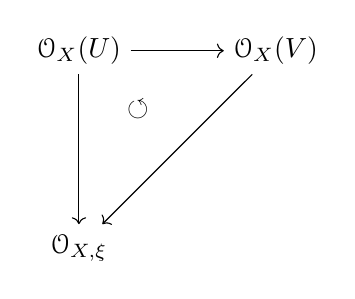
\begin{tikzpicture}[auto]
      \node (OU) at (0,0) {$\mathcal{O}_{X}(U)$};
      \node (Oxi) at (0,-2.5) {$\mathcal{O}_{X,\xi}$};
      \node (OV) at (2.5,0) {$\mathcal{O}_{X}(V)$};
      \node (ci) at (0.75,-0.75) {$\circlearrowleft$};

      \draw[->] (OU) to node () {} (OV);
      \draw[->] (OU) to node () {} (Oxi);
      \draw[->] (OV) to node () {} (Oxi);
    \end{tikzpicture}
  \end{center}
  が可換となるので,制限は単射である.
}

\Lemma{
$X = \text{Spec}\, A$をアフィンスキームとし,$g\in A$をとる.このとき開集合$D(g)$は
$X$から誘導される局所環付き空間で$\spec{A_{g}}$に同型なアフィンスキームになる.
}{
$Y = \spec{A_{g}}$と置く.局所化と素イデアルの対応より標準的な開はめ込み
\begin{equation*}
  i:Y \to X
\end{equation*}
がある($\im i = D(g)$)\\
$D(h)\subset D(g)$とする.$A\stackrel{\varphi}{\longrightarrow} A_{g}$とする.また$\varphi(h) = \bar{h}$と置く.このとき標準的な同型
\begin{equation*}
  \mathcal{O}_{X}(D(h)) = A_{h} \simeq (A_{g})_{\bar{h}} = \mathcal{O}_{Y}(D(\bar{h})) = i_{*}\mathcal{O}_{Y}(D(h))
\end{equation*}
今$A_{h}\simeq (A_{g})_{\bar{h}}$は感覚的には
\begin{equation*}
  (A_{g})_{\bar{h}} = (A[1/g])_{\bar{h}} = A[1/g,1/\bar{h}]
\end{equation*}
で,$D(h)\subset D(g)$より$h^{n} = gb$となる$n\in \mathbf{N}-\{0\}$と$b\in A$がある.よって
\begin{equation*}
  A[1/g,1/\bar{h}] = A[b/h^{n},1/\bar{h}] = A[1/h]=A_{h}
\end{equation*}
具体的にはまず,$\varphi$が単射ではないとき,
\begin{equation*}
  \ker{\varphi} \neq 0 \Leftrightarrow A_{g} = 0
\end{equation*}
に注意すると(よって$(A_{g})_{\bar{h}} = 0$),定義から$\ker{\varphi} \ni a \neq 0$とすると
\begin{equation*}
  \exists m\in \mathbf{N}\text{ s.t. } g^{m}a = 0
\end{equation*}
を満たす.また$h^n = gb$より$h^{nm}a = g^{m}ab^{m} = 0$より$\ker{(A\to A_{h})}$は$0$でない.
従って,$A_{h}=0$だから自明に同型である.よって$\varphi$を単射とする.\\
\begin{equation*}
  (A_{g})_{\bar{h}} \to A_{h}
\end{equation*}
を,
\begin{equation*}
  \frac{a}{g^{m}}\frac{1}{\bar{h}^{k}} \mapsto \frac{ab^{m}}{h^{mn}}\frac{1}{h^{k}} = \frac{ab^{m}}{h^{mn + k}}
\end{equation*}
で定義する.これは簡単に準同型で$0\leq k<n$としてよい.次に
\begin{equation*}
  A_{h} \to (A_{g})_{\bar{h}}
\end{equation*}
を,
\begin{equation*}
  \frac{a}{h^{n}} \mapsto \frac{\bar{a}}{\bar{h}^{n}}
\end{equation*}
ただし,$0\leq k<n$とする.これらは互いに逆射を与えるので,
$\{D(h)\}_{h}$は$D(g)$の開基となるので,$i$は$(Y,\mathcal{O}_{Y})$から$(D(g),\mathcal{O}_{X}|_{D(g)})\subset (X,\mathcal{O}_{X})$
への同型を誘導する.(Refer to Exercises 2.7)
}

\Definition{
\index{すきーむ@スキーム}\index{scheme}
\textbf{スキーム(scheme)}とは局所環付き空間$(X,\mathcal{O}_{X})$で開被覆$\{U_{i}\}_{i}$に対して$(U_{i},\mathcal{O}_{X}|_{U_{i}})$
がアフィンスキームになるものが存在するときをいう.また$\mathcal{O}_{X}(U)$の元は(やや不適切であるが)
\index{せいそくかんすう@正則関数}\index{regular function}
\textbf{$U$上の正則関数(regular functions on $U$)}という.しかし,層の関数としての側面をよく表している.(Refer to Exercises 3.4 and Proposition 4.4)
}

明らかにアフィンスキームはスキームである.また,局所環付き空間$X$が開被覆$\{U_{i}\}_{i}$に対して
$(U_{i},\mathcal{O}_{X}|_{U_{i}})$がスキームだったら$X$はスキームである.逆に次の命題が従う.

\Proposition{
$X$をスキームとする.このとき任意の開集合$U\subset X$に対して局所環付き空間$(U,\mathcal{O}_{X}|_{U})$はまたスキームになる.
}{
定義より$X = \bigcup_{i}U_{i}$で$U_{i}$は開集合で,アフィンスキームになるものがある.
$U\cap U_{i}$がスキームとなることを示せば十分である.
}

\Definition{
$X$をスキームとする.$U$を$X$の開集合とする.スキーム$(U,\mathcal{O}_{X}|_{U})$を$X$の
\index{かいぶぶんすきーむ@開部分スキーム}\index{open subscheme}
\textbf{開部分スキーム(open subscheme)}
更に$(U,\mathcal{O}_{X}|_{U})$がアフィンスキームになるとき$U$を
\index{あふぃんかいしゅうごう@アフィン開集合}\index{affine open subset}
\textbf{アフィン開集合(affine open subset)}という.
}

以下,$X$の開集合$U$はスキームの構造が与えられているとする.

\Definition{
  $X$をスキーム,$f\in \mathcal{O}_{X}(X)$とする.
  \begin{equation*}
    X_{f}:= \{x\in X\ |\ f_{x} \in \mathcal{O}^{\times}_{X,x}\}
  \end{equation*}
  ただし,$A^{\times}$は$A$の単元群である.(LiuのDefinition 3.11.では*の記号を用いている.)
}

次の条件を考えよう.

\begin{conditionbox}
  $X$は有限アフィン開被覆$\{U_{i}\}_{i}$があって$U_{i}\cap U_{j}$はまた有限アフィン開被覆を持つ.
\end{conditionbox}
便宜上この条件を条件Aと呼称する.



\Proposition{
$X$をスキームとし$f\in \mathcal{O}_{X}(X)$とする.このとき$X_{f}$は$X$の開集合で,
更に,$X$が条件Aを満たすなら,制限$\mathcal{O}_{X}(X)\to \mathcal{O}_{X}(X_{f})$は同型
\begin{equation*}
  \mathcal{O}_{X}(X)_{f} \simeq \mathcal{O}_{X}(X_{f})
\end{equation*}
を誘導する.
}{
$x\in X_{f}$とする.$x$の開近傍$U$と$g\in \mathcal{O}_{X}(U)$があって,$f_{x}g_{x} = 1$を満たすものがある.
$f_{x}g_{x} = (fg)_{x}$よりある$x$の開近傍$V\subset U$があって$fg|_{V}=1$を満たす.
したがって,$V\subset X_{f}$となる.よって$X_{f}$は開集合である.\\
更に,$V$が動くにつれて$f$の逆元$g\in \mathcal{O}_{X}(V)$を張り合わせると
$f|_{X_{f}}$の$\mathcal{O}_{X}(X_{f})$での逆元を得る.\\
詳しく言えば,$X_{f}$の上の$V$を集めた開被覆$\{V_{i}\}_{i}$を取り,$fg_{i}|_{V_{i}} = 1$なる$g_{i} \in \mathcal{O}_{X}(V_{i})$を考えれば
任意の$i,j$に対して
\begin{equation*}
fg_{i}|_{V_{i} \cap V_{j}} = 1 = fg_{j}|_{V_{i} \cap V_{j}}
\end{equation*}
より
\begin{align*}
(左辺) - (右辺) 
&= fg_{i}|_{V_{i} \cap V_{j}} - fg_{j}|_{V_{i} \cap V_{j}}\\
&= f|_{V_{i} \cap V_{j}}(g_{i}|_{V_{i} \cap V_{j}} - g_{j}|_{V_{i} \cap V_{j}})\\
&= 0
\end{align*}
また,$f|_{V_{i}}$は単元なので逆元$(f|_{V_{i}})^{-1}$がある.また,
\begin{equation*}
f|_{V_{i} \cap V_{j}} = (f|_{V_{i}})|_{V_{i} \cap V_{j}}
\end{equation*}
なので,
\begin{align*}
f|_{V_{i} \cap V_{j}} ((f|_{V_{i}})^{-1}|_{V_{i} \cap V_{j}}) 
&= (f|_{V_{i}})|_{V_{i} \cap V_{j}} ((f|_{V_{i}})^{-1}|_{V_{i} \cap V_{j}}) \\
&= ((f|_{V_{i}})(f|_{V_{i}})^{-1})|_{V_{i} \cap V_{j}} \\
&= 1
\end{align*}
よって$f|_{V_{i} \cap V_{j}}$はまた単元で$g_{i}|_{V_{i} \cap V_{j}} = g_{j}|_{V_{i} \cap V_{j}}$を得る.

$\mathcal{O}_{X}$は層なので,貼り合わせ条件より$g|_{V_{i}} = g_{i}$なる$g\in \mathcal{O}_{X}(X_{f})$がある.
この$g$が$f|_{X_{f}}$の逆元になっている.\\
よって制限$\mathcal{O}_{X}(X)\to \mathcal{O}_{X}(X_{f})$
から準同型
\begin{equation*}
\alpha : \mathcal{O}_{X}(X)_{f}\to \mathcal{O}_{X}(X_{f});\frac{x}{f^n} \mapsto \rho_{X,X_f}(x)f^{-n} = \rho_{X,X_f}(x)g^n
\end{equation*}
を誘導する.($\mathcal{O}_{X}(X)$は環なので$\mathcal{O}_{X}(X)_{f}$は$\{f^{n}\}_{n\in \mathbf{N}}$での局所化であることに注意しよう.)
ここで条件Aを仮定すれば,$X$は有限アフィン開被覆$\mathcal{U} = \{U_{i}\}_{i}$を持つ.
よって,
\begin{equation*}
X_{f} = \bigcup_{i}U_{i}\cap X_{f} = \bigcup_{i}V_{i} = \bigcup_{i}D(f|_{U_{i}})
\end{equation*}
ここで,$U_{i} = \spec{A_{i}}$とすると
\begin{align*}
  U_{i} \cap X_{f} 
  &= \{x\in X\cap \spec{A_{i}}\mid f_{x} \in \mathcal{O}_{X,x}^{\times}\}\\
  &= \{x\in \spec{A_{i}}\mid f_{x} \in \mathcal{O}_{X,x}^{\times}\}\\
  &= \{x\in \spec{A_{i}}\mid f_{x} \in (\mathcal{O}_{X}|_{\spec{A_{i}},x})^{\times}\}\\
  &= \{\mathfrak{p}\in \spec{A_{i}}\mid f_{\mathfrak{p}} \in A_{i,\mathfrak{p}}^{\times}\}
\end{align*}
ここで,素イデアルの局所化$A_{\mathfrak{p}}$が局所環でその極大イデアルが
$A_{\mathfrak{p}}\mysetminus A_{\mathfrak{p}}^{\times} = \mathfrak{p}A_{\mathfrak{p}}$となることに注意すると
\begin{align*}
  \{\mathfrak{p} \in \spec{A_{i}}\mid f_{\mathfrak{p}}\in A_{i,\mathfrak{p}}^{\times}\}
  &= \{\mathfrak{p} \in \spec{A_{i}} \mid f_{\mathfrak{p}} \notin \mathfrak{p}A_{i,\mathfrak{p}}\}\\
  &= \{\}
\end{align*}
%D(f|_{U_{i}})がなぞ
Lem:\ref{Lem:1.5.3}より$\mathcal{O}_{X}(U_{i})_{f} = \mathcal{O}_{X}(V_{i})$\\
今以下の完全系列を得る.
\begin{equation*}
C^{\bullet}(\mathcal{U},\mathcal{O}_{X}):0 \longrightarrow \mathcal{O}_{X}(X) \stackrel{d_{0}}{\longrightarrow} \bigoplus_{i}\mathcal{O}_{X}(U_{i}) \stackrel{d_{1}}{\longrightarrow} \bigoplus_{i,j}\mathcal{O}_{X}(U_{i} \cap U_{j})
\end{equation*}
ただし$d_{0}:s\mapsto (s|_{U_{i}})_{i},d_{1}:(s_{i})_{i}\mapsto (s_{i}|_{U_{i}\cap U_{j}} - s_{j}|_{U_{i} \cap U_{j}})_{i,j}$
とする.(有限個なら直積$\prod$と直和$\bigoplus$は同じ)\\
次にテンソルをとることは左完全関手なので$C^{\bullet}(\mathcal{U},\mathcal{O}_{X})\otimes_{\mathcal{O}_{X}(X)}\mathcal{O}_{X}(X)_{f}$
はまた,完全列である.よってこれは次の可換図式を与える.

\begin{center}
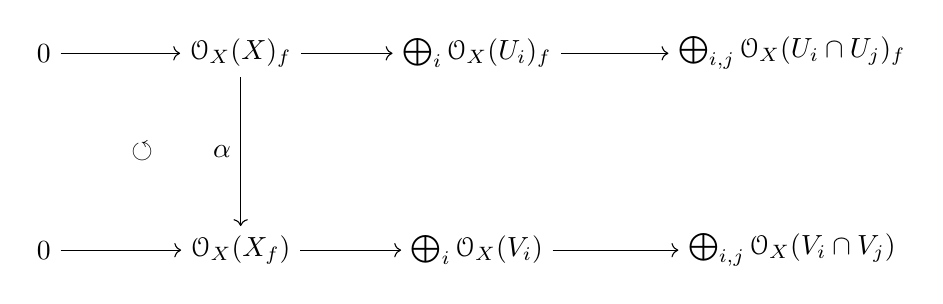
\begin{tikzpicture}[auto]
  \node (00) at (0,0) {$0$};
  \node (01) at (0,-2.5) {$0$};
  \node (OX_f) at (2.5,0) {$\mathcal{O}_{X}(X)_{f}$};
  \node (OXf_) at (2.5,-2.5) {$\mathcal{O}_{X}(X_{f})$};
  \node (oOU_f) at (5.5,0) {$\bigoplus_{i}\mathcal{O}_{X}(U_{i})_{f}$};
  \node (oOV) at (5.5,-2.5) {$\bigoplus_{i}\mathcal{O}_{X}(V_{i})$};
  \node (oOUU_f) at (9.5,0) {$\bigoplus_{i,j}\mathcal{O}_{X}(U_{i}\cap U_{j})_{f}$};
  \node (oOVV) at (9.5,-2.5) {$\bigoplus_{i,j}\mathcal{O}_{X}(V_{i}\cap V_{j})$};
  \node (ci) at (1.25,-1.25) {$\circlearrowleft$};

  \draw[->] (00) to (OX_f);
  \draw[->] (01) to (OXf_);
  \draw[->] (OX_f) to (oOU_f);
  \draw[->] (OXf_) to (oOV);
  \draw[->] (oOU_f) to (oOUU_f);
  \draw[->] (oOV) to (oOVV);
  \draw[->] (OX_f) to node[label=left:$\alpha$] () {} (OXf_);
  % \draw[->] (X2) to node[yshift = -2pt,label=below:$f_{\lambda}$] () {} (Y2);
  % \draw[->] (Y1) to node[xshift = -6pt,label=right:$\psi_{\lambda,\mu}$] () {} (Y2);
\end{tikzpicture}
\end{center}
}

\subsection{Morphism of schemes}
\Definition{
  \index{すきーむ@スキーム!のしゃ@の射}\index{scheme!morphism}
  $f:X\to Y$が\textbf{スキームの射(morphism of schemes)}とは局所環付き空間としての射とする.
}

環の射$\varphi:A\to B$が誘導する射$\spec{B} \to \spec{A}$を$\varphi^{a}$と書くことにする.\\
つまり$\mathfrak{p}\in \spec{B}$に対して$\varphi^{a}(\mathfrak{p}) = \varphi^{-1}(\mathfrak{p})$

\Proposition{
  $\varphi: A \to B$を環の射とする.このとき
  \begin{equation*}
    (\varphi^{a},(\varphi^{a})^{\#}):\spec{B} \to \spec{A}
  \end{equation*}
  は$(\varphi^{a})^{\#}(\spec{A})=\varphi$を満たすスキームの射である.
}{
  $X=\spec{B},Y=\spec{A}$と置く.任意の$f\in A$に対して
  \begin{equation*}
    (\varphi^{a})^{-1}(D(f))=D(\varphi(f))
  \end{equation*}
  が成り立ち,実際
  \begin{align*}
    (\varphi^{a})^{-1}(D(f)) 
    &= \{ \mathfrak{p} \in X\ |\ \varphi^{a}(\mathfrak{p}) \in D(f)\}\\
    &= \{ \mathfrak{p} \in X\ |\ f \notin \varphi^{a}(\mathfrak{p})\}\\
    &= \{ \mathfrak{p} \in X \mid f \notin \varphi^{-1}(\mathfrak{p})\}\\
    &= \{ \mathfrak{p} \in X \mid \varphi(f) \notin \mathfrak{p}\}\\
    &= D(\varphi(f))
  \end{align*}  
  である.$\varphi$から誘導される環の射
  \begin{equation*}
    (\varphi^{a})^{\#}(D(f)):\mathcal{O}_{Y}(D(f)) = A_{f} \to B_{\varphi(f)} = \mathcal{O}_{X}(D(\varphi(f))) = (\varphi^{a})_{*}\mathcal{O}_{X}(D(f))
  \end{equation*}
  これは制限写像と可換(compatibleという意味で)になる.よって層の射
  \begin{equation*}
    (\varphi^{a})^{\#}:\mathcal{O}_{Y} \to \varphi^{a}_{*}\mathcal{O}_{X}
  \end{equation*}
  に拡張できる.
  %開基?(or 基本開集合族)で決まっていれば拡張できることを証明する.
  更に,任意の$\mathfrak{q} \in X$に対して$\varphi$から誘導される環の射
  \begin{equation*}
    (\varphi^{a})^{\#}_{\mathfrak{q}}:A_{\varphi^{a}(\mathfrak{q})} \to B_{\mathfrak{q}}
  \end{equation*}
  は局所射で,実際
  \begin{align*}
    (\varphi^{a})^{\#}_{\mathfrak{q}}(\varphi^{a}(\mathfrak{q})A_{\varphi^{a}(\mathfrak{q})})
    &= \{ \varphi(a)/\varphi(p) \mid a\in \varphi^{a}(\mathfrak{q}),p \notin \varphi^{a}(\mathfrak{q})\}\\
    &= \{\varphi(a)/\varphi(p)\mid \varphi(a)\in \mathfrak{q},\varphi(p)\notin \mathfrak{q}\}\\
    &\subset \{b/q\mid b\in \mathfrak{q},q\notin \mathfrak{q}\}\\
    &= \mathfrak{q}B_{\mathfrak{q}}
  \end{align*}
  よって$(\varphi^{a},(\varphi^{a})^{\#})$は
  局所環付き空間の射になる.構成により
  \begin{equation*}
    (\varphi^{a})^{\#}(Y):\mathcal{O}_{Y}(Y) = A \to B = \mathcal{O}_{X}(X) = (\varphi^{a})_{*}\mathcal{O}_{X}(Y)
  \end{equation*}
  で$(\varphi^{a})^{\#}(Y) = \varphi$を満たす.
}

\Lemma{
  $A$を環とし,$I$をそのイデアルとする.このとき,スキームの射
  \begin{equation*}
    i:\spec{A/I} \to \spec{A}
  \end{equation*}
  が自然な射影$\varphi:A\to A/I$によって誘導される.$i$は$\im{i} = V(I)$へのスキームの閉はめ込みである.
  更に,任意の$\spec{A}$の基本開集合$D(f)$に対して
  \begin{equation*}
    (\ker{i^{\#}})(D(f)) = I\otimes_{A}A_{f}
  \end{equation*}
  が成り立つ.
}{
  $i$が閉はめ込みであることはよい.次に,任意の$\spec{A}$の基本開集合$D(f)$に対して先ほど
  みたように,標準的な全射
  \begin{equation*}
    \mathcal{O}_{\spec{A}}(D(f)) = A_{f} \to (A/I)_{\varphi(f)} = i_{*}\mathcal{O}_{\spec{A/I}}(D(f))
  \end{equation*}
  がある.これにより,$i^{\#}$の全射性と,
  \begin{align*}
    (\ker{i^{\#}})(D(f)) 
    &= \ker{(i^{\#}(D(f)))}\\
    &= \ker{(A_{f} \to (A/I)_{\varphi(f)})}\\
    &= I_{f} \\
    &= I\otimes_{A}A_{f}
  \end{align*}
  がわかる.
}

\Definition{
  $Z$を$X$の閉集合とする.このとき$Z$が
  \index{へいぶぶんすきーむ@閉部分スキーム}\index{closed subscheme}
  \textbf{閉部分スキーム(closed subscheme)}とは
  包含写像$j:Z\to X$が閉はめ込み
  \begin{equation*}
    (j,j^{\#}):(Z,\mathcal{O}_{Z}) \to (X,\mathcal{O}_{X})
  \end{equation*}
  となるときをいう.
}



\Proposition{
  $X=\spec{A}$をアフィンスキームとする.$j:Z\to X$をスキームの閉はめ込みとする.
  このとき,$Z$はアフィンスキームで,あるイデアル$J\subset A$が唯一存在して
  $j$は同型$Z\stackrel{\simeq}{\longrightarrow}\spec{A/J}$を誘導する.
}{}

\Definition{
  $S$をスキームとする.このとき$X$が
  \index{えすすきーむ/えすじょうのすきーむ@$S$-スキーム/$S$上のスキーム}
  \index{S-scheme/scheme over S@$S$-scheme/scheme over $S$}
  \textbf{$S$-スキーム($S$-scheme)}または\textbf{$S$上のスキーム(scheme over $S$)}とは
  スキームの射$\pi:X \to S$が与えられているときをいう.この$\pi$を
  \index{こうぞうしゃ@構造射}\index{structural morphism}
  \textbf{構造射(structural morphism,\ structure morphism)}
  ,$S$を
  \index{きていすきーむ@基底スキーム}\index{base scheme}
  \textbf{基底スキーム(base scheme)}という.
}

スキーム$X,Y$に対して
\begin{equation*}
  \hom{\textbf{Sch}}{X}{Y}:=\{f:X\to Y\ |\ f\text{ is morphism of schemes}\}
\end{equation*}
また,環$A,B$に対して
\begin{equation*}
  \hom{\textbf{Ring}}{A}{B}:=\{f:A\to B\ |\ f\text{ is morphism of rings}\}
\end{equation*}
とおく.このとき標準的な写像
\begin{equation*}
  \rho:\hom{\textbf{Sch}}{X}{Y} \to \hom{\textbf{Ring}}{\mathcal{O}_{Y}(Y)}{\mathcal{O}_{X}(X)}
\end{equation*}
がある.実際$(f,f^{\#})\in \hom{\textbf{Sch}}{X}{Y}$とすると
\begin{equation*}f^{\#}(Y):\mathcal{O}_{Y}(Y) \to f_{*}\mathcal{O}_{X}(Y) = \mathcal{O}_{X}(f^{-1}(Y))=\mathcal{O}_{X}(X)
\end{equation*}
がある.
%関手的であることを確認する.



\clearpage
\appendix
\chapter{Limit}

\Section{Inductive Limit}
とりあえず,帰納極限だけ述べる.射影極限は双対概念なのでまぁ頑張って.
\Definition{(帰納系の定義)\\
($\Lambda,\leq$)を順序集合,$\mathscr{C}$を圏とする.各$\lambda \in \Lambda$に対し,$X_{\lambda} \in \text{Ob}(\mathscr{C})$が与えられ,
$\lambda \leq \mu$に対して射$\varphi_{\mu,\lambda}:X_{\lambda} \to X_{\mu}$があって
次を満たすとき,$\{X_{\lambda},\varphi_{\mu,\lambda}\}$を\textbf{順系(direct system)}または
\textbf{帰納系(inductive system)}という.しばし$\varphi_{\mu,\lambda}$を省略して$\{X_{\lambda}\}_{\lambda \in \Lambda}$や$\{X_{\lambda}\}_{\lambda}$で表す.
\begin{itemize}
  \item[---] 任意の$\lambda \in \Lambda$に対して$\varphi_{\lambda,\lambda}=\text{id}_{X_{\lambda}}$
  \item[---] $\lambda \leq \mu \leq \nu$なる任意の$\lambda,\mu,\nu \in \Lambda$に対して$\varphi_{\nu,\lambda} = \varphi_{\nu,\mu}\circ \varphi_{\mu,\lambda}$
\end{itemize}
}
\Example{
位相空間$X$の開集合族$\{U\}_{U}$に対して
\begin{equation*}
  U \leq V \defi V \subset U
\end{equation*}
と定義する.そして,$\mathbf{AGrp}$をアーベル群の成す圏,$\mathcal{F}$を$X$上の前層とする.すると,各開集合$U$に対し,$\mathcal{F}(U) \in \mathrm{Ob}(\mathbf{AGrp})$で,
前層の定義からアーベル群と制限写像との組$\{\mathcal{F}(U),\rho_{U,V}\}$は帰納系となる.前層の定義はDef:\ref{Def:1.3.1}を参照.
}{}
\Definition{(帰納系の射の定義)\\
$\Lambda$を順序集合.$\{X_{\lambda},\varphi_{\lambda,\mu}\},\{Y_{\lambda},\psi_{\lambda,\mu}\}$を$\Lambda$上の圏$\mathscr{C}$における帰納系とする.
このとき$\{X_{\lambda}\}$から$\{Y_{\lambda}\}$への射とは$f_{\lambda}:X_{\lambda} \to Y_{\lambda}$なる射の族
$\{f_{\lambda}\}$で,任意の$\lambda \leq \mu$に対して
$\psi_{\lambda,\mu}\circ f_{\mu} = f_{\lambda}\circ \varphi_{\lambda,\mu}$となるものを言う.
%---------------後に図式を追加する.------------------%
\begin{center}
\begin{tikzpicture}[auto]
  \node (X1) at (0,0) {$X_{\mu}$};
  \node (X2) at (0,-2.5) {$X_{\lambda}$};
  \node (Y1) at (2.5,0) {$Y_{\mu}$};
  \node (Y2) at (2.5,-2.5) {$Y_{\lambda}$};
  \node (ci) at (1.25,-1.25) {$\circlearrowleft$};

  \draw[->] (X1) to node[yshift = -6pt,label=above:$f_{\mu}$] () {} (Y1);
  \draw[->] (X1) to node[label=left:$\varphi_{\lambda,\mu}$] () {} (X2);
  \draw[->] (X2) to node[yshift = -2pt,label=below:$f_{\lambda}$] () {} (Y2);
  \draw[->] (Y1) to node[xshift = -6pt,label=right:$\psi_{\lambda,\mu}$] () {} (Y2);
\end{tikzpicture}
\end{center}
}
\Definition{
$\mathscr{C}$を圏とし,$\Lambda$を順序集合とする.$\{X_{\lambda},\varphi_{\mu,\lambda}\}$を
$\mathscr{C}$の帰納系とする.\\
このとき$\{X_{\lambda},\varphi_{\mu,\lambda}\}$の\textbf{順極限(direct limit)}または\textbf{帰納的極限(inductive limit)}または\textbf{帰納極限}とは,
$\mathscr{C}$の対象$\displaystyle \varinjlim_{\lambda \in \Lambda}X_{\lambda} \in \text{Ob}(\mathscr{C})$
と射の族$\displaystyle \{\varphi_{\lambda}:X_{\lambda} \to \varinjlim_{\lambda \in \Lambda}X_{\lambda}\}_{\lambda \in \Lambda}$の組
$\{\varinjlim X_{\lambda},\varphi_{\lambda}\}$で,次の条件を満たすものをいう.
\begin{itemize}
\item[---] $\lambda \leq \mu$に対して$\varphi_{\mu}\circ \varphi_{\mu,\lambda} = \varphi_{\lambda}$
\item[---] $\lambda \leq \mu$に対して$f_{\mu}\circ \varphi_{\mu,\lambda} = f_{\lambda}$を満たす任意の射の族$\{f_{\lambda}:X_{\lambda} \to Y\}_{\lambda \in \Lambda}$に対して,
      $\displaystyle f:\varinjlim_{\lambda \in \Lambda}X_{\lambda} \to Y$が一意に存在して
      \begin{equation*}
        f\circ \varphi_{\lambda} = f_{\lambda}\quad (\forall \lambda \in \Lambda)
      \end{equation*}
      を満たす.
\end{itemize}
}
\Remark{
一般の圏では帰納極限や射影極限は存在するとは限らない.しかし,存在するとすれば,同型を除いて一意である.
}{}
\Proposition{
帰納極限は存在すれば,同型を除いて一意である.
}{
証明は後で書く.
}


\printindex
\end{document}